\section{Planejamento de Projeto}

Para melhor entender as etapas de desenvolvimento, antes é preciso conhecer o contexto do problema que deu origem ao processo de idealização, definição de interface e fluxo de execução da ferramenta. \\

\textbf{Processo de idealização} \\

Atualmente, para que clientes façam o uso de estruturas de dados remotos, estes precisam encontrar um meio de buscá-los eventualmente antes de executar uma lógica que dependa dos dados. Isso sugere a escrita de um código encarregado de acessar serviços\footnote{
  Infraestrutura distribuída (servidores, banco de dados, etc) que responde à pedidos de operações oriundas de clientes em forma de requisições de API.
} em busca de dados pela rede.

No entanto, para que haja garantia na comunicação, ao buscar dados diretamente em pontos de acesso\footnote{
  Parte de uma interface exposta por um serviço através de um canal de comunicação.
} de uma API, cria-se um contrato de acesso entre o cliente e a interface do serviço. Isso porque, uma vez implementado o código de busca, é preciso uma garantia de que não haja mudanças que ponham em risco sua funcionalidade e, assim, comprometer parte da lógica da aplicação. Além de possíveis danos financeiros, perde-se tempo de desenvolvimento de reimplementação.

\begin{figure}[H]
  \centering
  \begin{tikzpicture}[font=\small]
    \node (client) at (-3,0) {\includegraphics[width=1.0cm]{figuras/client}};
    \node[right of=client] (clientFetchCode) at (-2.2,0.7) {\includegraphics[width=1.1cm]{figuras/code}};
    \node[below of=clientFetchCode, node distance=1.6cm] (clientLogicCode) {\includegraphics[width=1.1cm]{figuras/code}};
    \node[rectangle,minimum width=0.8cm, minimum height=3cm,draw,right of=clientFetchCode, node distance=3.0cm] (api) {API};
    \node[right of=api, node distance=1.8cm] (server) {\includegraphics[width=1.0cm]{figuras/server}};
    \node[below of=server, node distance=1.8cm] (datastore) {\includegraphics[width=1.0cm]{figuras/database}};
    \node[above of=server, node distance=1.8cm] (json) {\includegraphics[width=1.1cm]{figuras/code}};
    \node[cloud, cloud puffs=30, minimum width=11cm, minimum height=10cm, draw,style={scale=0.6}] (service) at (server) {};
    \node[below of=clientFetchCode,node distance=0.0cm] {\textless$busca$\textgreater};
    \node[below of=clientLogicCode,node distance=0.0cm] {\textless$logica$\textgreater};
    \node[below of=json,node distance=0.0cm] {\{data\}};
    \node[below of=service,node distance=3.6cm] {Serviço};
    \node[below of=client,node distance=1.8cm] {\ldots};
    \node[right of=server,node distance=1.8cm] {\ldots};
    \draw[decorate,decoration={brace,raise=0.2cm,mirror}] ([yshift=6pt]clientFetchCode.north west) -- ([yshift=-12pt]clientLogicCode.south west);
    \draw [->] ([yshift=0.25cm]clientFetchCode.east) -- ([yshift=0.25cm]api.west);
    \draw [->] (api) -- (clientFetchCode);
  \end{tikzpicture}
  \caption{Contrato entre cliente e serviço na busca de dados}
\end{figure}

Atualmente, um dos problemas mais comuns de quebra de contrato entre API's e clientes ocorre em serviços que implementam o estilo de arquitetura REST. Em REST, pequenas mudanças como a de fluxo de dados\footnote{
  Fluxo de acesso do cliente em pontos de acesso para a busca de uma representação da estrutura total do serviço.
} podem causar instabilidade e o versionamento desnecessário de sua interface. Já em arquiteturas como GraphQL, o risco para esse tipo de mudança é baixo, pois não limita na interface a forma que clientes façam o acesso em busca de dados.

Vale lembrar que existem mudanças de diferentes níveis de impacto e complexidade de resolução. Por exemplo, mudanças como a de fluxo de dados ou estilo de arquitetura são possíveis de serem evitadas, pois afetam apenas o código de busca. Já mudanças como a alteração de campos da estrutura de dados são mais difíceis de serem resolvidas, pois seu acoplamento vai além do código de busca, podendo estar presente na lógica da aplicação.

\begin{figure}[H]
  \centering
  \begin{tikzpicture}[font=\small]
    \draw (-2,0) -- (-2,-5) (2,0) -- (2,-5);
    \node at (-2,0.3) {Cliente};
    \node at (2,0.3) {API (Serviço)};
    \node[dashed] (virtualData) at (-4,-1){\includegraphics[width=1.1cm]{figuras/code}};
    \node[below of=virtualData,node distance=0.0cm] {\{data\}};
    \node (data) at (-4,-4.5) {\includegraphics[width=1.1cm]{figuras/code}};
    \node[below of=data,node distance=0.0cm] {\{data\}};
    \node[cloud, cloud puffs=16,draw,minimum height=1.2cm] (cloudData) at (4,-2.5) {\includegraphics[width=1.1cm]{figuras/code}};
    \node[below of=cloudData,node distance=0.0cm] {\{data\}};
    \draw[->] (-2,-1) -- node[midway,above] {requisição} (2,-1.5);
    \draw[<-] (-2,-2.5) -- node[midway,above] {resposta} (2,-2);
    \draw[->] (-2,-3) -- node[midway,above] {requisição} (2,-3.5);
    \draw[<-] (-2,-4.5) -- node[midway,above] {resposta} (2,-4);
  \end{tikzpicture}
  \caption{Fluxo de dados}
\end{figure}


\begin{figure}[H]
  \centering
  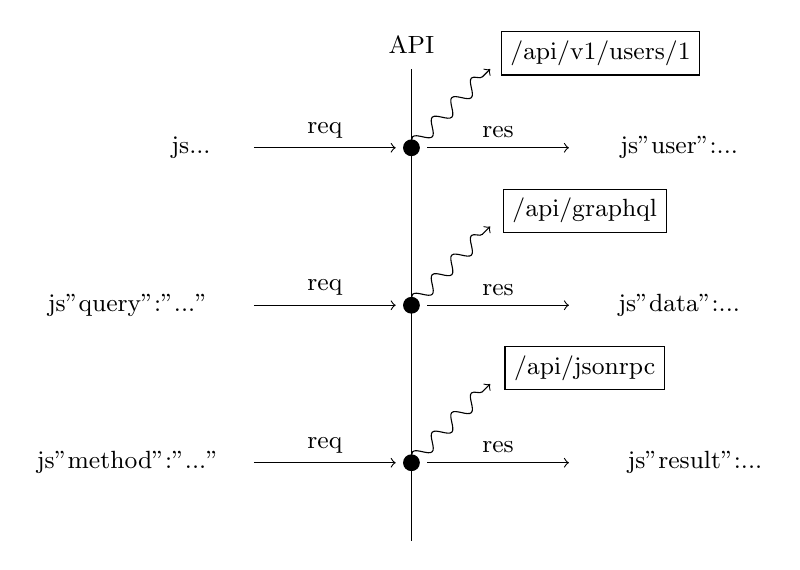
\begin{tikzpicture}[font=\small]
    \draw (0,1) -- (0,-5);
    \node at (0,1.3) {API};
    \node[draw,shape=circle,fill=black,style={scale=0.6}] at (0,0) {};
    \node[draw,shape=circle,fill=black,style={scale=0.6}] at (0,-2) {};
    \node[draw,shape=circle,fill=black,style={scale=0.6}] at (0,-4) {};
	\node at (-2.8,0) {\mintinline{js}{{...}}};
    \node at (-3.6,-2) {\mintinline{js}{{"query":"..."}}};
    \node at (-3.6,-4) {\mintinline{js}{{"method":"..."}}};
	\node at (3.4,0) {\mintinline{js}{{"user":{...}}}};
    \node at (3.4,-2) {\mintinline{js}{{"data":{...}}}};
    \node at (3.6,-4) {\mintinline{js}{{"result":{...}}}};
    \draw[->] (-2,0) -- node[midway,above] {req} (-0.2,0);
    \draw[->] (-2,-2) -- node[midway,above] {req} (-0.2,-2);
    \draw[->] (-2,-4) -- node[midway,above] {req} (-0.2,-4);
    \draw[->] (0.2,0) -- node[midway,above] {res} (2,0);
    \draw[->] (0.2,-2) -- node[midway,above] {res} (2,-2);
    \draw[->] (0.2,-4) -- node[midway,above] {res} (2,-4);
    \draw[->,decorate,decoration={snake,post length=1mm}] (0,0) -- (1,1);
    \draw[->,decorate,decoration={snake,post length=1mm}] (0,-2) -- (1,-1);
    \draw[->,decorate,decoration={snake,post length=1mm}] (0,-4) -- (1,-3);
    \node[draw] at (2.4,1.2) {/api/v1/users/1};
    \node[draw] at (2.2,-0.8) {/api/graphql};
    \node[draw] at (2.2,-2.8) {/api/jsonrpc};
  \end{tikzpicture}
  \caption{Requisição e resposta para estilos de arquitetura}
\end{figure}

A fim de melhorar a comunicação entre clientes e serviços através da possível prevenção de mudanças que levam a quebra de contrato, antes, fez-se necessário solucionar uma série de problemas descritos a seguir.
 
\begin{enumerate}
\item \textbf{Problema}: Dificuldade de realizar mudanças no fluxo de dados e estilo de arquitetura de uma API sem interferir no código de busca de clientes. \\ \textbf{Solução}: Encontrar uma ferramenta para uso no cliente que evite o contrato de acesso nesses casos.
\item \textbf{Problema}: Não encontrado uma ferramenta para a resolução do problema anterior. \\ \textbf{Solução}: Construir uma ferramenta para clientes que faça a intermediação na comunicação entre seu código de busca e API do serviço.
\item \textbf{Problema}: Criar uma linguagem para usar na comunicação entre código de busca e ferramenta para depois transformar em requisições de API. \\ \textbf{Solução}: Usar a linguagem GraphQL para expressar consulta de dados e depois analisar sintaxe a fim de transformar em requisições.
\item \textbf{Problema}: Encontrar uma estrutura para se trabalhar com a sintaxe das consultas GraphQL descritas em texto. \\ \textbf{Solução}: Converter a sintaxe das consultas em texto em estruturas AST\footnote{
  Árvores sintáticas abstratas
} para análise de dependências de dados.
\item \textbf{Problema}: Converter AST's em requisições para API's de serviços. \\ \textbf{Solução}: Análise de metadados em pontos de acesso através de arquivos de descrição de API.
\item \textbf{Problema}: Escolher requisições de menor tempo de resposta para acesso de dados do cliente. \\ \textbf{Solução}: Algoritmo que analisa AST's e metadados de API's em busca o menor número de pontos de acesso e avalia o tamanho de resposta como critério.
\end{enumerate}

Após solucionar os problemas, é proposto o primeiro protótipo do projeto onde prevê a criação de uma ferramenta que faça a intermediação na comunicação entre código de busca do cliente e API do serviço. Além disso, será necessário a reimplementação do código de busca para linguagem GraphQL, um arquivo para descrição da API disponibilizado pelo serviço e outro no cliente para configuração da ferramenta.

\begin{figure}[H]
  \centering
  \begin{tikzpicture}[font=\small]
    \node (client) at (-3,0) {\includegraphics[width=1.0cm]{figuras/client}};
    \node[right of=client] (clientFetchCode) at (-2.2,0) {\includegraphics[width=1.1cm]{figuras/code}};
    \node[below of=clientFetchCode, node distance=1.6cm] (clientLogicCode) {\includegraphics[width=1.1cm]{figuras/code}};
    \node[above of=clientFetchCode, node distance=1.6cm] (clientConfigCode) {\includegraphics[width=1.1cm]{figuras/code}};
    \node[circle,draw,right of=clientFetchCode,node distance=2.3cm] (schema) {Ferramenta};
    \node[rectangle,minimum width=0.8cm, minimum height=3cm,draw,node distance=1.8cm,right of=schema,node distance=2.7cm] (api) {API};
    \node[right of=api, node distance=1.8cm] (json) {\includegraphics[width=1.1cm]{figuras/code}};
    \node[below of=json,node distance=1.8cm] (server) {\includegraphics[width=1.0cm]{figuras/server}};
    \node[above of=json, node distance=1.8cm] (description) {\includegraphics[width=1.1cm]{figuras/code}};
    \node[cloud, cloud puffs=30, minimum width=11cm, minimum height=10cm, draw,style={scale=0.6}] (service) at (json) {};
    \node[below of=clientFetchCode,node distance=0.0cm] {\textless$busca$\textgreater};
    \node[below of=clientLogicCode,node distance=0.0cm] {\textless$logica$\textgreater};
    \node[below of=clientConfigCode,node distance=0.0cm] {\textless$config$\textgreater};
    \node[below of=description,node distance=0.0cm] {\{desc\}};
    \node[below of=json,node distance=0.0cm] {\{data\}};
    \node[below of=service,node distance=3.6cm] {Serviço};
    \node[below of=client,node distance=1.8cm] {\ldots};
    \node[right of=json,node distance=1.8cm] {\ldots};
    \draw[decorate,decoration={brace,raise=0.2cm,mirror}] ([yshift=6pt]clientConfigCode.north west) -- ([yshift=-12pt]clientLogicCode.south west);
    \draw [->] ([yshift=0.25cm]clientFetchCode.east) -- ([yshift=0.25cm]schema.west);
    \draw [->] (schema) -- (clientFetchCode);
    \draw [->] ([yshift=0.25cm]schema.east) -- ([yshift=0.25cm]api.west);
    \draw [->] (api) -- (schema);
    \path [line,dashed] (clientConfigCode) -| ([xshift=-0.25cm]schema.north);
    \path [line,dashed] (description) -| ([xshift=0.25cm]schema.north);
  \end{tikzpicture}
  \caption{Proposta de modelo para evitar quebra de contrato}
\end{figure}

O novo modelo de comunicação procura, além de evitar a quebra de contrato, proporcionar um ambiente escalável para a composição de dados através de serviços baseados em JSON. Podendo ser aplicado em outras áreas de dificuldade como na adoção de novos estilos de arquiteturas e busca de dados em micro-serviços.

\begin{figure}[H]
  \centering
  \begin{tikzpicture}[font=\small]
    \node (client1) at (-2,0) {\includegraphics[width=1.0cm]{figuras/client}};
    \node (client2) at (2,0) {\includegraphics[width=1.0cm]{figuras/client}};
    \node[circle,draw,below of=client2,node distance=2.3cm] (schema) {Ferramenta};
    \node[cloud, cloud puffs=16, draw] (service1) at (-3,-6) {Serviço 1};
    \node[cloud, cloud puffs=16, draw] (service2) at (0,-6) {Serviço 2};
    \node[cloud, cloud puffs=16, draw] (service3) at (3,-6) {Serviço 3};
    \node[right of=service3,node distance=2.8cm] {\ldots};
    \draw [<->] (client1) -- (service1);
    \draw [<->] (client1) -- (service2);
    \draw [<->] (client1) -- (service3);
    \draw [<->] (client2) -- (schema);
    \draw [<->] (schema) -- (service1);
    \draw [<->] (schema) -- (service2);
    \draw [<->] (schema) -- (service3);
  \end{tikzpicture}
  \caption{Composição de serviços sem e com o modelo proposto}
\end{figure}

\textbf{Definição de interface} \\

Para introduzir a ferramenta em um ambiente de clientes em produção, é importante oferecer uma interface que apresente uma baixa curva de aprendizagem e que cause pouco impacto no código existente. A ideia de utilizar GraphQL como principal linguagem de comunicação serve não apenas para poupar desenvolvimento mas também incentivar o seu uso de forma que o código de busca não fique dependente da ferramenta. Assim, clientes GraphQL podem ser desenvolvidos de forma gradual, onde não há a necessidade de implementar um interpretador GraphQL no serviço caso faça o uso da ferramenta. 

Outro caso é trabalhar com formatos abertos para descrição de API's, como por exemplo em REST o JSON Hyper-Schema. Isso permite agilizar a integração da ferramenta com serviços que já oferecem alguma solução completa para descrição de sua API's e que existe uma forma (adaptador) da ferramenta entender esses metadados.

Ao integrar a ferramenta no código clientes, é preciso definir um arquivo de configuração contendo funções que descreva informações de cada serviço a ser consultado. Após, gera-se um esquema GraphQL pela ferramenta a partir das funções de configuração de serviço. Por fim, é executado no código de busca as consultas através do esquema gerado.

\begin{figure}[H]
  \centering
  \begin{minted}[frame=single,framesep=10pt,fontsize=\small]{javascript}
    import {adapter} from "graphql-jay-hyperschema"
  
    export function v1() {
      return fetch("/api/v1/schema").then((response) => {
        return response.json()
      }).then((schema) => {
        return {
          url: "/api/v1",
          schema,
          adapter,
          wrapper: {}
        }
      })
    }
  \end{minted}
  \caption{Exemplo de função de configuração para serviço REST}
\end{figure}

\begin{figure}[H]
  \centering
  \begin{minted}[frame=single,framesep=10pt,fontsize=\small]{javascript}
    import {graphql} from "graphql"
    import {composeSchema} from "graphql-jay"
    import services from "./services"
    
    composeSchema(...services).then((schema) => {
      graphql(schema, "{ user { id } }").then((response) => { 
        console.log(response.data)
      })
    })
  \end{minted}
  \caption{Exemplo de criação de esquema e execução de consulta}
\end{figure}

\textbf{Fluxo de execução} \\

Ao a efetuar a busca de dados entre clientes e serviços utilizando a ferramenta, dois fluxos de execução são realizados. O primeiro é o processo criação de esquema, que recebe como entrada funções de configuração de serviços e retorna um esquema GraphQL. O segundo é o processo de consulta de dados, onde a leva como entrada consultas em texto GraphQL e retorna estruturas de dados JSON remotas.

\begin{figure}[H]
  \centering
  \begin{tikzpicture}[font=\small]
    \node [block] (composeSchema) {Compõe esquema};
    \node [oval, above of=composeSchema,node distance=2cm] (services) {Serviços};
    \node [block, right of=composeSchema,node distance=3cm] (buildSchema) {Constrói esquemas de serviços};
    \node [block, right of=buildSchema,node distance=3cm] (wrapSchema) {Invólucro esquemas de serviços};
    \node [block, right of=wrapSchema,node distance=3cm] (deepExtendSchema) {Extende esquemas de serviços};
    \node [oval, above of=deepExtendSchema,node distance=2cm] (schema) {Esquema};
    \path [line] (composeSchema) -- (buildSchema);
    \path [line] (buildSchema) -- (wrapSchema);
    \path [line] (wrapSchema) -- (deepExtendSchema);
    \path [line,dashed] (services) -- (composeSchema);
    \path [line,dashed] (deepExtendSchema) -- (schema);
  \end{tikzpicture}
  \caption{Criação de esquema}
\end{figure}

\begin{figure}[H]
  \centering
  \begin{tikzpicture}[font=\small]
    \node [block] (simplifyAST) {Simplifica AST};
    \node [oval, above of=simplifyAST,node distance=2cm] (services) {Consulta};
    \node [block, below of=simplifyAST,node distance=2cm] (transformAST) {Transforma ASTs de serviços};
    \node [block, right of=transformAST,node distance=3cm] (reduceASTs) {Reduz ASTs de serviços};
    \node [block, right of=reduceASTs,node distance=3cm] (unwrapAST) {Desfazer invólucro de ASTs};
    \node [block, right of=unwrapAST,node distance=3cm] (fetchData) {Busca dados};
    \node [block, above of=fetchData,node distance=2cm] (wrapData) {Invólucro dados};
    \node [oval, above of=wrapData,node distance=2cm] (schema) {Dados};
    \draw [->] (simplifyAST) -- (transformAST);
    \draw [->] (transformAST) -- (reduceASTs);
    \draw [->] (reduceASTs) -- (unwrapAST);
    \draw [->] (unwrapAST) -- (fetchData);
    \draw [->] (fetchData) -- (wrapData);
    \draw [->,dashed] (services) -- (simplifyAST);
    \draw [->,dashed] (wrapData) -- (schema);
  \end{tikzpicture}
  \caption{Consulta de dados}
\end{figure}

